\documentclass{article}

\usepackage{amsmath,amssymb}
\usepackage{tikz}
\usepackage{pgfplots}
\usepackage{xcolor}
\usepackage[left=2.1cm,right=3.1cm,bottom=3cm,footskip=0.75cm,headsep=0.5cm]{geometry}
\usepackage{enumerate}
\usepackage{enumitem}
\usepackage{marvosym}
\usepackage{tabularx}
\usepackage[amsmath,thmmarks,standard]{ntheorem}
\usepackage{mathtools}

\usepackage[utf8]{inputenc}

\renewcommand*{\arraystretch}{1.4}
\newcommand{\E}{\mathbb{E}}

\newcolumntype{L}[1]{>{\raggedright\arraybackslash}p{#1}}
\newcolumntype{R}[1]{>{\raggedleft\arraybackslash}p{#1}}
\newcolumntype{C}[1]{>{\centering\let\newline\\\arraybackslash\hspace{0pt}}m{#1}}

\DeclareMathOperator{\tr}{tr}
\DeclareMathOperator{\Var}{Var}
\DeclareMathOperator{\Cov}{Cov}
\renewcommand{\E}{\mathbb{E}}

\newtheorem{thm}{Theorem}
\newtheorem{lem}{Lemma}

\title{\textbf{Einführung in die Produktion, Hausaufgabe 7}}
\author{\textsc{Henry Haustein}}
\date{}

\begin{document}
	\maketitle
	
	\section*{Aufgabe 7}
	\begin{enumerate}[label=(\alph*)]
		\item Es handelt sich um ein offenes Lager, da die Produkte sofort weitergegeben werden. Zudem haben wir eine Produktionsgeschwindigkeit von $\frac{50}{\text{min}}$ und eine Verbrauchsgeschwindigkeit von $\frac{40}{\frac{1}{2}\text{min}}=\frac{80}{\text{min}}$. Es handelt sich also um ein offenes Zerreißlager.
		\item Diagramm:
		\begin{center}
			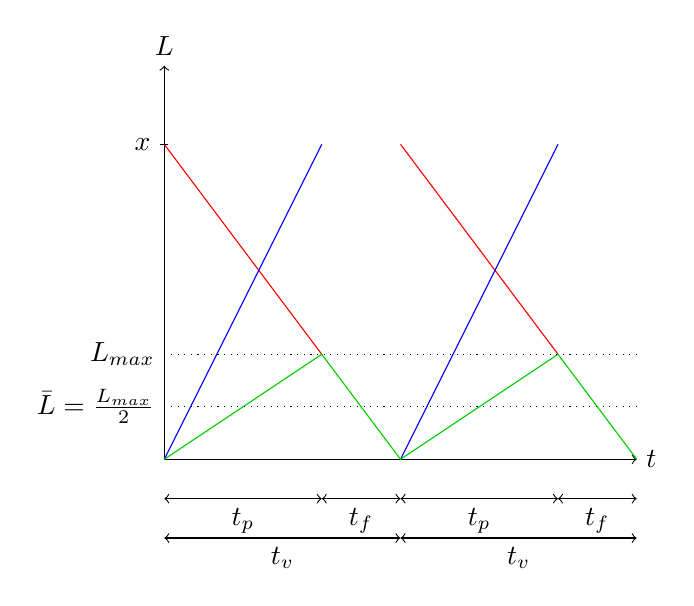
\begin{tikzpicture}
				\draw[->] (0,0) -- (6,0) node[right] {$t$};
				\draw[->] (0,0) -- (0,5) node[above] {$L$};
				
				\draw[red] (0,4) -- (2,4/3);
				\draw[red] (3,4) -- (5,4/3);
				\draw[blue] (0,0) -- (2,4);
				\draw[blue] (3,0) -- (5,4);
				\draw[green!80!black] (0,0) -- (2,4/3) -- (3,0) -- (5,4/3) -- (6,0);
				
				\draw[dotted] (0,4/3) node[left] {$L_{max}$} -- (6,4/3);
				\draw[dotted] (0,2/3) node[left] {$\bar{L}=\frac{L_{max}}{2}$} -- (6,2/3);
				\draw (-0.05,4) node[left] {$x$} -- (0.05,4);
				
				\draw[<->] (0,-0.5) to node[midway,below] {$t_p$} (2,-0.5);
				\draw[<->] (2,-0.5) to node[midway,below] {$t_f$} (3,-0.5);
				\draw[<->] (0,-1) to node[midway,below] {$t_v$} (3,-1);
				\draw[<->] (3,-0.5) to node[midway,below] {$t_p$} (5,-0.5);
				\draw[<->] (5,-0.5) to node[midway,below] {$t_f$} (6,-0.5);
				\draw[<->] (3,-1) to node[midway,below] {$t_v$} (6,-1);
			\end{tikzpicture} \\
			\textcolor{blue}{Produktion}, \textcolor{red}{Verbrauch}, \textcolor{green!80!black}{Lagerbestandsverlauf}
		\end{center}
	\item Lagerhaltungskosten je Los:
	\begin{align}
		K_{L,Los} &= \frac{L_{max}}{2} \cdot t_v \cdot c_L \notag \\
		L_{max} &= t_p(x_p-x_v) \notag \\
		&= \frac{x}{x_p}(x_p-x_v) \notag \\
		&= x\left(1-\frac{x_v}{x_p}\right) \notag \\
		t_v &= \frac{x}{x_v} \notag \\
		K_{L,Los} &= \frac{x}{2}\left(1-\frac{x_v}{x_p}\right) \cdot \frac{x}{x_v}\cdot c_L \notag \\
		&= \frac{x^2}{2}\left(\frac{1}{x_v}-\frac{1}{x_p}\right)\cdot c_L \notag
	\end{align}
	\item Multiplikation mit der Losauflagehäufigkeit $n=\frac{B}{x}$ ergibt:
	\begin{align}
		K_L &= \frac{x}{2}\left(\frac{1}{x_v}-\frac{1}{x_p}\right)\cdot c_L\cdot B \notag
	\end{align}
	Gesamtkosten sind also (als $k_R$ sind bei einem Staulager immer die Rüstkosten der ersten Maschine zu benutzen, also $k_R=k_{R,I}$)
	\begin{align}
		K(x) &= K_L + K_R \to\min \notag \\
		&= \frac{x}{2}\left(\frac{1}{x_v}-\frac{1}{x_p}\right)\cdot c_L\cdot B + k_R\frac{B}{x} \to\min \notag
	\end{align}
	\item Ableiten und Nullsetzen
	\begin{align}
		\frac{\partial K}{\partial x} = \frac{1}{2}\left(\frac{1}{x_v}-\frac{1}{x_p}\right)\cdot c_L\cdot B - k_R\frac{B}{x^2} &= 0 \notag \\
		\frac{1}{2}\left(\frac{1}{x_v}-\frac{1}{x_p}\right)\cdot c_L\cdot B &= k_R\frac{B}{x^2} \notag \\
		x_{opt} &= \sqrt{\frac{2k_R}{\left(\frac{1}{x_v}-\frac{1}{x_p}\right)\cdot c_L}} \notag
	\end{align}
	\end{enumerate}
	
\end{document}